\documentclass[a4paper]{article}

\author{14231016 马琛骁}
\title{San Fransisco Crime Report}

\usepackage{xeCJK}
\setCJKmainfont{Songti SC}
\usepackage{indentfirst}

\usepackage{listings}

\usepackage[superscript]{cite}
\makeatletter % changes the catcode of @ to 11
\renewcommand\@citess[1]{\textsuperscript{[#1]}}
\makeatother % changes the catcode of @ back to 12

\begin{document}

\maketitle

\section{数据概览}

训练数据共有 878049 条,每条有 9 个属性,分别统计这些属性值的可能选项如下:

\begin{table}[h]
    \centering
    \begin{tabular}{*{10}{r}}
        \hline
        Total & Date & Cate & Dspt & DOW & Pd & Res & Add & X & Y \\
        \hline
        878049 & 389257 & 39 & 879 & 7 & 10 & 17 & 23228 & 34243 & 34243 \\
        1 & 2 & 22514 & 999 & 125436 & 87805 & 51650 & 38 & 26 & 26 \\
        \hline
    \end{tabular}
    \caption{训练集属性值的取值范围和每种取值的平均样本数}
\end{table}

测试数据共有 65499 条,每条有 6 个属性,分别统计这些属性值的可能选项如下:

\begin{table}[h]
    \centering
    \begin{tabular}{*{7}{r}}
        \hline
        Total & Date & DOW & Pd & Add & X & Y \\
        \hline
        65499 & 28495 & 7 & 10 & 12124 & 13925 & 13925 \\
        1 & 2 & 9357 & 6550 & 5 & 5 & 5 \\
        \hline
    \end{tabular}
    \caption{测试集属性值的取值范围和每种取值的平均样本数}
\end{table}

接下来统计各个属性在训练集和测试集的重合度。

\begin{figure}[h]
    \centering
    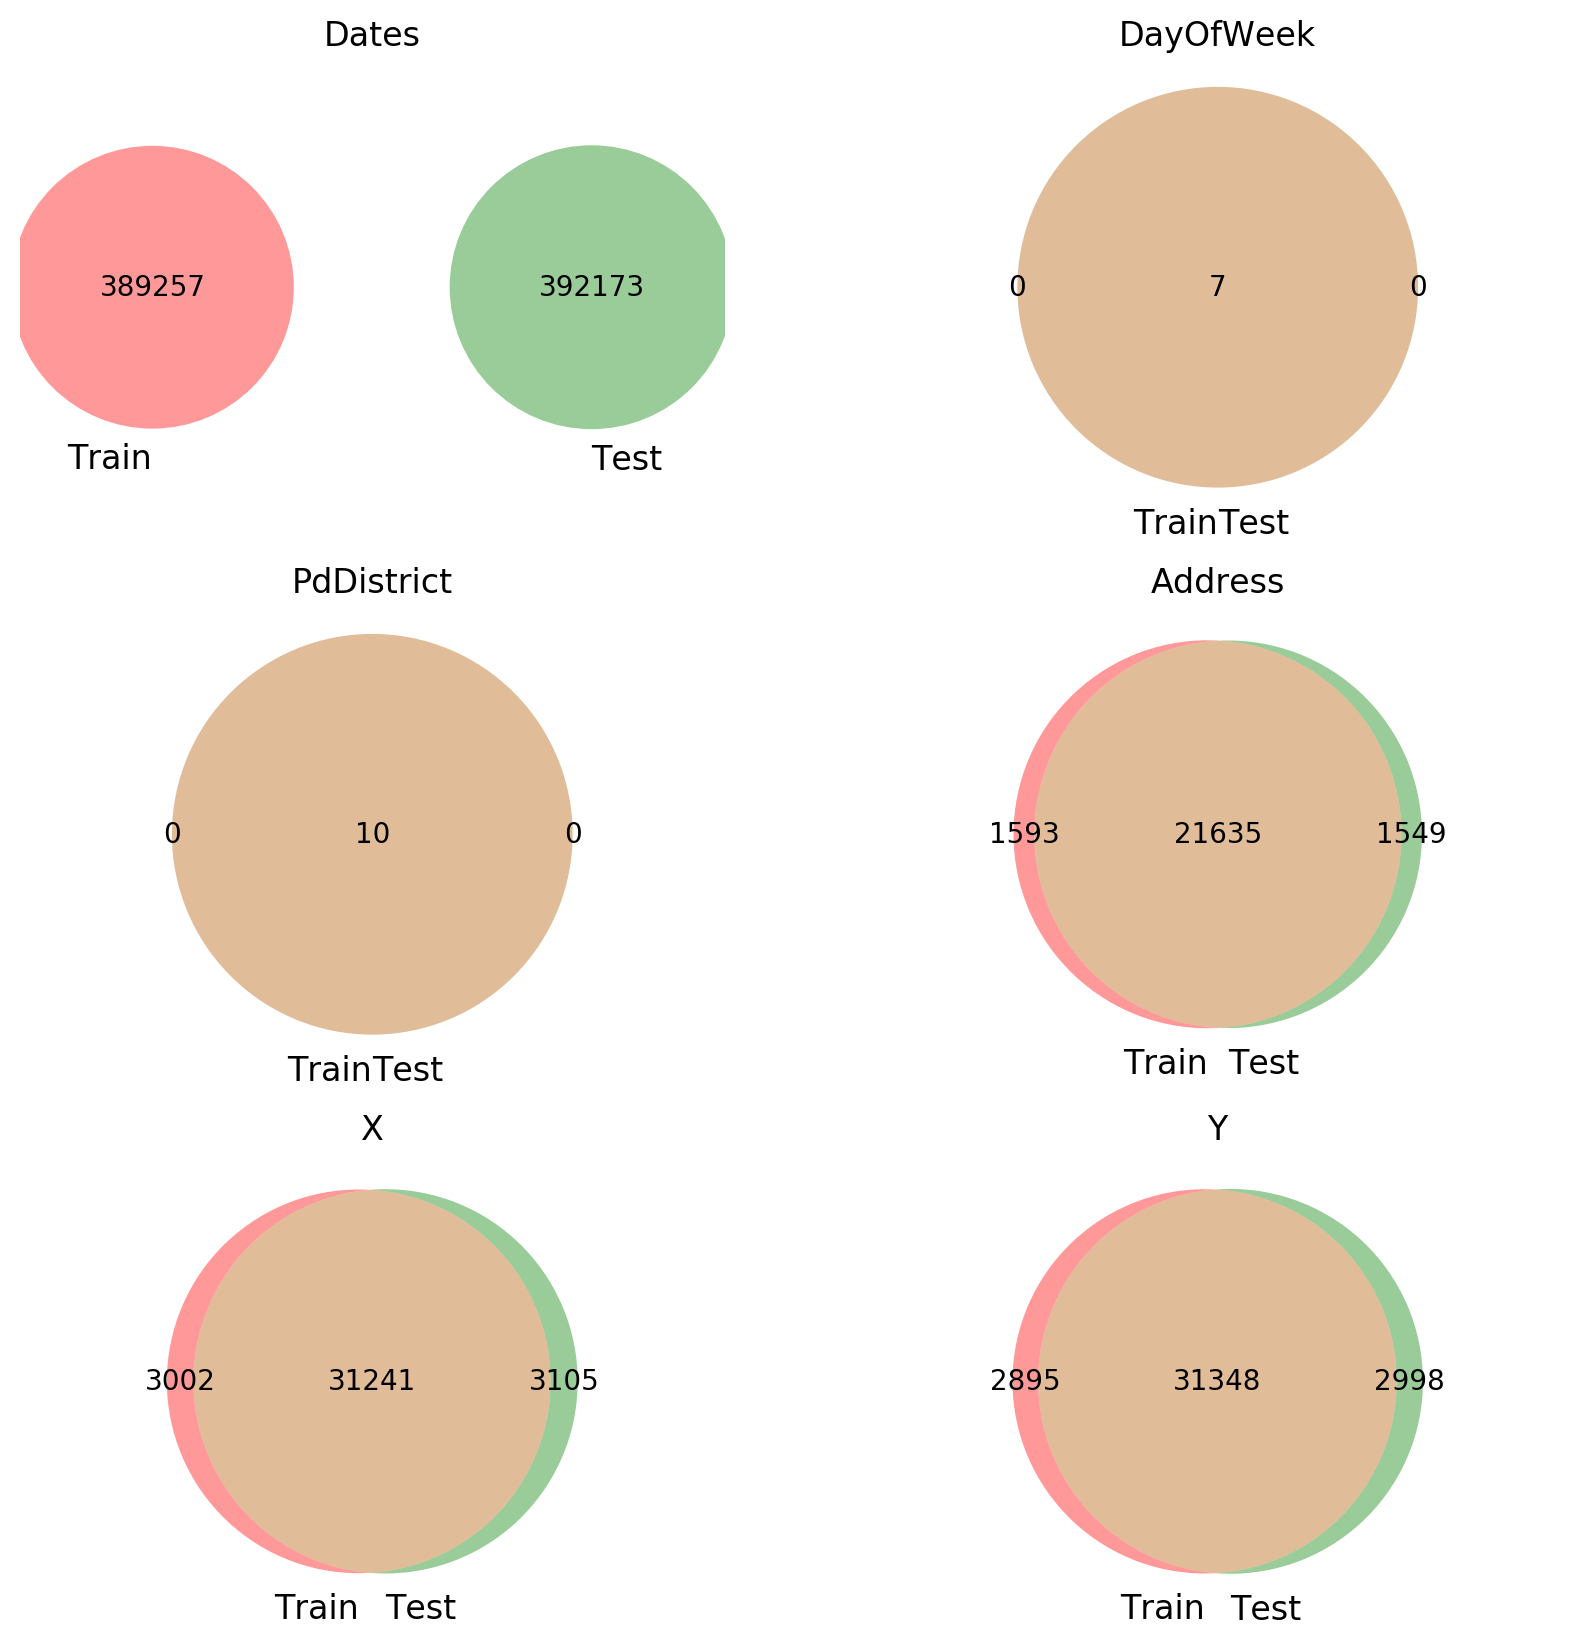
\includegraphics[width=\textwidth]{overlap.png}
    \caption{属性重合度}
\end{figure}

注意到测试集和训练集的日期完全没有重合,
因此考虑将日期分割为“小时”,“日”,“月”,“年”四个属性,
经过统计,此时训练集和测试集完全重合。

\begin{figure}[h]
    \centering
    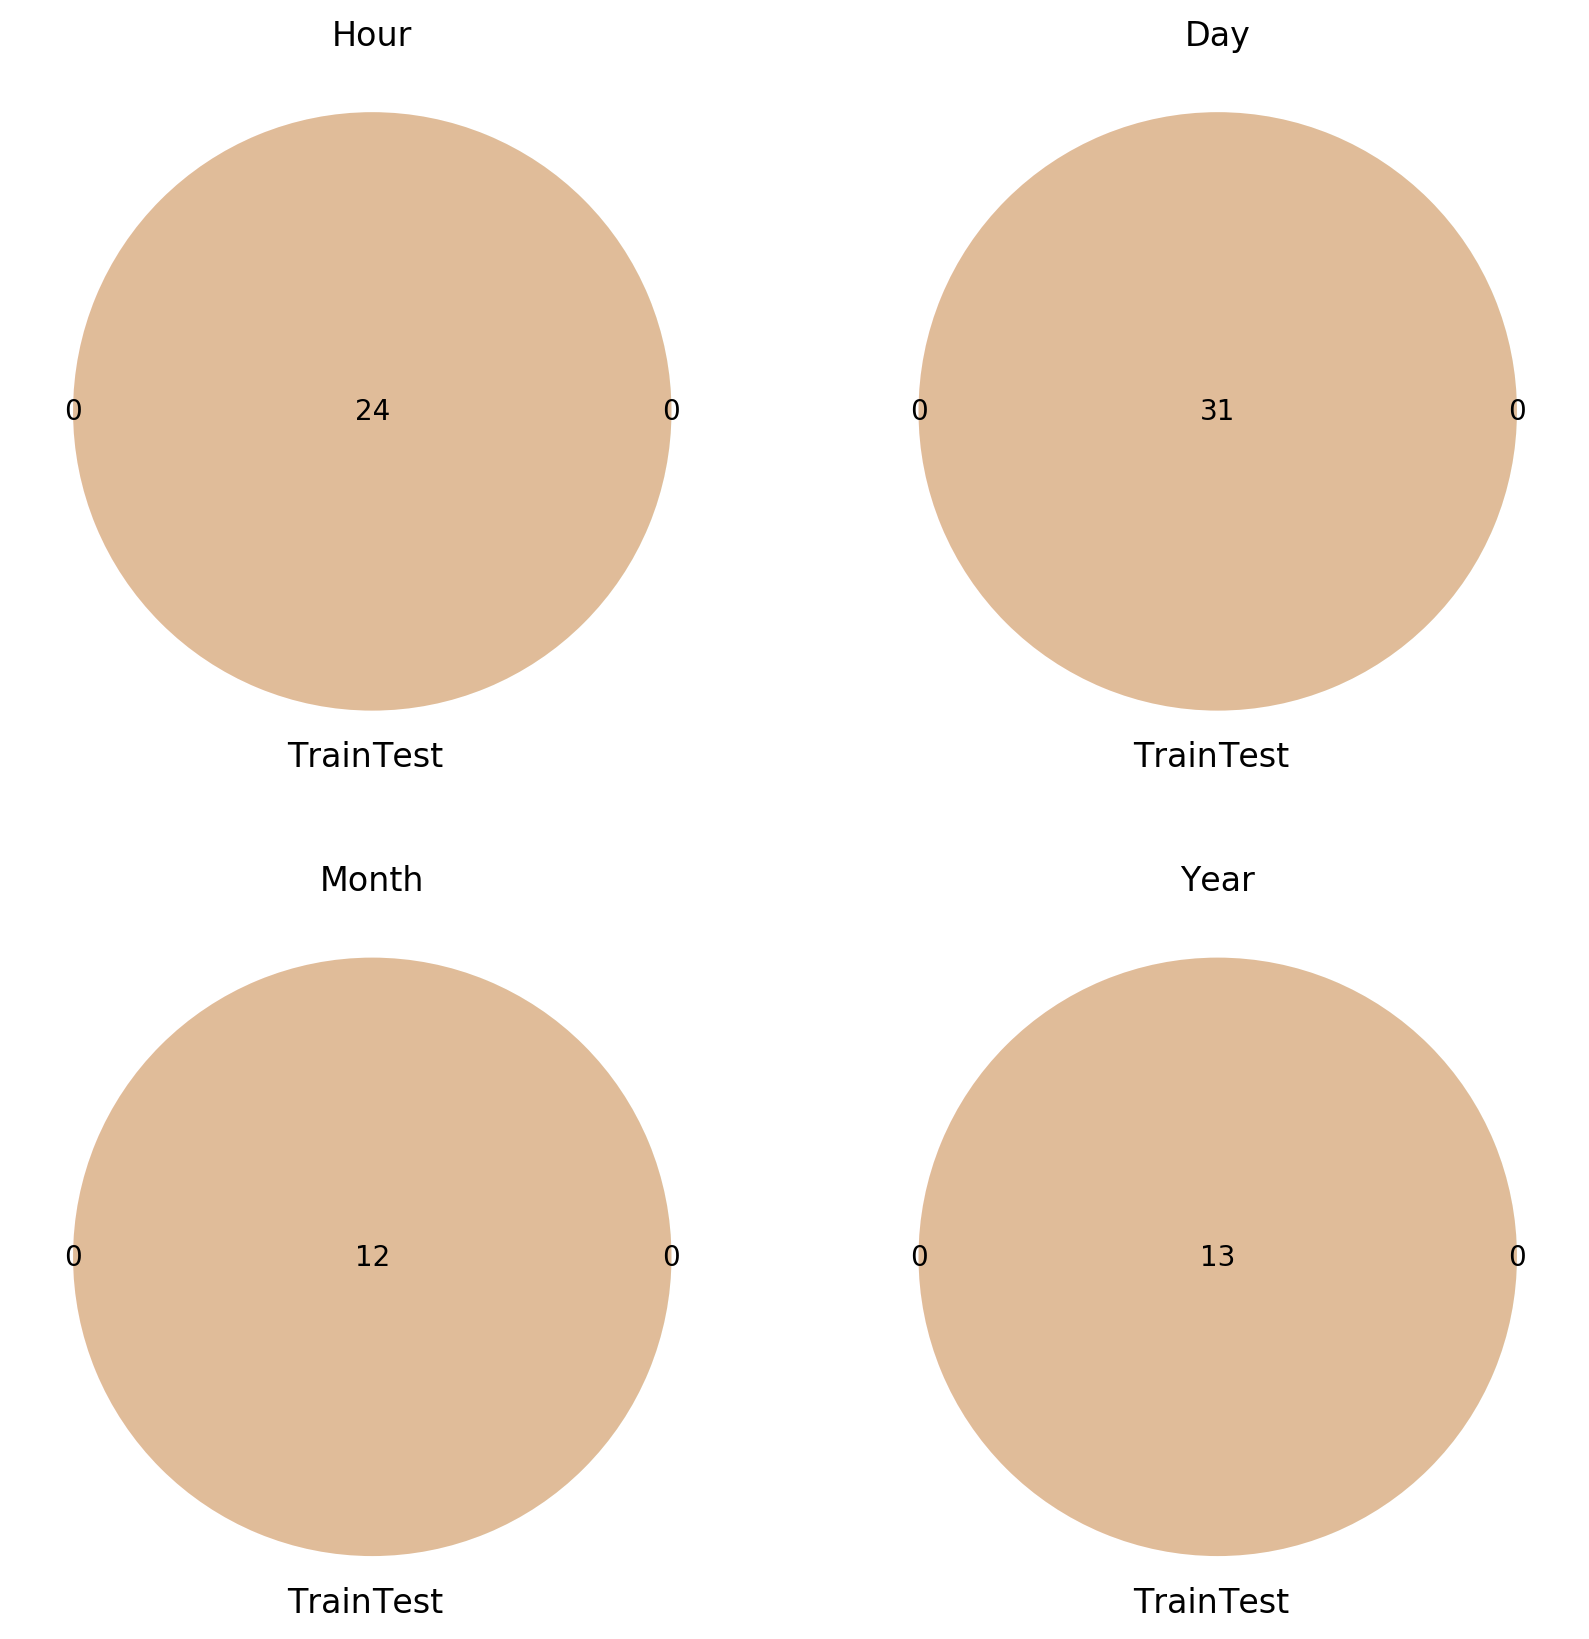
\includegraphics[width=\textwidth]{overlap_2.png}
    \caption{细分属性重合度}
\end{figure}

\section{决策树}

决策树是一种机器学习模型,
它通过对训练数据进行分析,得到一个多次选择的分类器,
每一次根据样本的某个或某些属性进行决策,最终得到样本的分类。
决策树的每一个内部节点是样本的某一个特征,
从这个节点出发的每一个弧表示这个特征的可能取值,
如果指向另一个内部节点,则表示需要对另外一个样本特征进行决策,
如果指向叶子结点,则表示已经得到了对样本分类的结论。

与一个训练集不矛盾的决策树可能存在多个,也可能不存在,
因此需要定义评价函数来衡量决策树的性能。
常用的评价函数有信息增益(Information Gain)和基尼指数(Gini Impurity)等。

使用Scikit Learn库中的 \lstinline[basicstyle=\ttfamily]|DecisionTreeClassifier|
进行训练及预测。

\section{结果}

\begin{table}[h]
    \centering
    \begin{tabular}{cc}
        \hline
        模型 & 结果 \\
        \hline
        决策树 & 23 \\
        \hline
    \end{tabular}
\end{table}

\bibliography{main}{}
\bibliographystyle{plain}

\end{document}

